\section{Introdução \label{sec:introducao}}

\subsection{\textit{Smooth} em imagens}

Neste trabalho é implementado um algoritmo para fazer \textit{smooth} em um imagem no formato PPM P3. Nesta seção é explicado o formato de arquivo PPM P3 e como funciona o algoritmo para aplicar o efeito \textit{smooth}. Na Seção~\ref{sec:desenvolvimento}, é explicado o desenvolvimento da modelagem do problema e codificação. Na Seção~\ref{sec:resultados}, resultados são apresentados e analisados. Por fim, é descrita uma conclusão sobre a realização deste trabalho na Seção~\ref{sec:conclusao}.

Este relatório faz parte de um conjunto de arquivos referentes ao trabalho. A documentação do código-fonte encontra-se nos arquivos \texttt{.c} dentro de \texttt{./src} a partir do diretório raiz.

\subsection{O Formato PPM P3}

O formato de arquivo PPM P3 consiste em representar os dados de uma imagem em um arquivo ASCII. O cabeçalho do arquivo contém a palavra ``P3'' seguida de dois valores que representam a largura e comprimento da imagem e de um valor que representa o valor máximo para cada pixel da imagem. Por exemplo, o seguinte cabeçalho diz que a imagem tem 800px de largura, 600px de altura e que os pixels tem valor máximo de 255:

\texttt{P3} \\
\indent\texttt{800 600} \\
\indent\texttt{255}

Após o cabeçalho, seguem os valores das componentes \textit{Red, Green, Blue} (RGB) de cada pixel da imagem. No exemplo acima, após o valor 255, seguem $800 \times 600 \times 3 = 1 440 000$ valores, sendo a cada três referente a um componente RGB de um pixel.

\subsection{O Algoritmo \label{sec:algoritmo}}

O algoritmo aplicado consiste em: dada como entrada uma imagem de dimensões $w \times h$, para cada pixel $p_i = (R_i, G_i, B_i)$, $i = 0, 1, \dots, w h - 1$ da imagem, montar um bloco de pixels $B_i = (b_{i,0}, b_{i,1}, \dots, b_{i,24})$ de área $5 \times 5 = 25$ tomando $b_{i,12}$ = $p_i$ como pixel central desse bloco e os demais $b_{i,j \neq 12}$ como os pixels ao redor de $p_i$ na imagem de modo a compor a área do bloco. Caso não exista valor para algum $b_{i,j}$, se assume $b_{i,j} = (0,0,0)$.

Então é feita a média aritmética dos valores de cada pixel de $B_i$ e o resultado é atribuído ao pixel $p_i$ na imagem. Uma ilustração desse processo é mostrada na Figura~\ref{fig:ilustracao}.
\begin{equation}
	p_i = \frac{\sum_{j = 0}^{24} b_{i,j}}{25} \text{ , } i = 0, 1, \dots, w h - 1 \label{eq:aritmetica}
\end{equation}

% inkscape -D -z --file=./input/smooth.svg --export-pdf=./input/smooth.pdf

\begin{figure}[h]
	\centering
	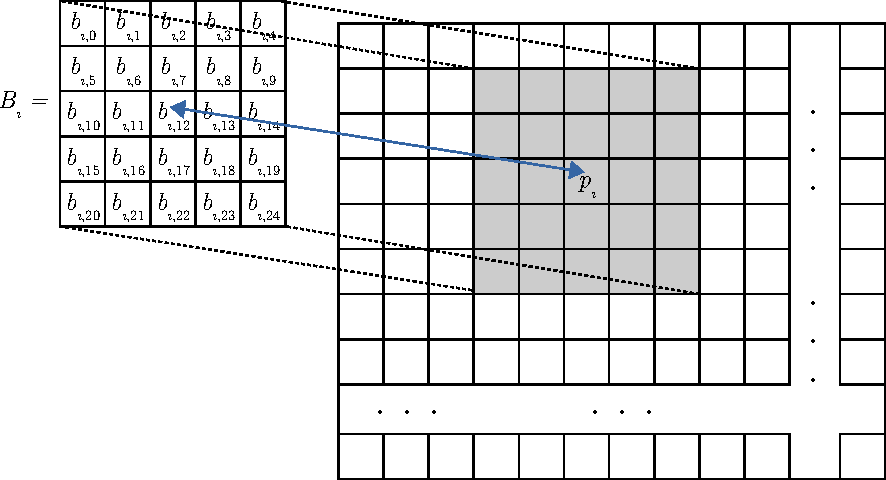
\includegraphics[scale=1]{./input/smooth.pdf}
	\caption{Ilustração da aplicação de \textit{smooth} em um pixel $p_i$ de uma imagem. \label{fig:ilustracao}}
\end{figure}


